%% Beispiel-Präsentation mit LaTeX Beamer im KIT-Design
%% entsprechend den Gestaltungsrichtlinien vom 1. August 2020
%%
%% Siehe https://sdqweb.ipd.kit.edu/wiki/Dokumentvorlagen

%% Beispiel-Präsentation
\documentclass{sdqbeamer}
\usepackage{booktabs}
\usepackage{graphicx}
\usepackage{xcolor}
\usepackage{listings}
\usepackage{tikz}
\usepackage{amssymb}


\lstdefinelanguage{GitLog}{
  morekeywords={feat,fix,chore,ci,Merge,draft},
  sensitive=false,
  morecomment=[l]{\#}
}

\lstset{
  language=GitLog,
  basicstyle=\ttfamily,
  keywordstyle=\color{blue},
  commentstyle=\color{gray},
  breaklines=true,
  columns=fullflexible,
  frame=single,
  keepspaces=true,
}

\AtBeginSection[]{
  \begin{frame}
  \vfill
  \centering
  \begin{beamercolorbox}[]{title}
    \centering\usebeamerfont{title}\huge\underline\insertsectionhead\par%
  \end{beamercolorbox}
  \vfill
  \end{frame}
}


%% Titelbild
\titleimage{banner_2020_kit}

%% Gruppenlogo
%\grouplogo{mylogo}

%% Gruppenname und Breite (Standard: 50 mm)
\groupname{Human-Computer Interaction and Accessibility}
\groupnamewidth{50mm}
\grouplogo{grouplogo.jpg}

% Beginn der Präsentation

\title[Solidarische Raumnutzung Abschlusspräsentation]{SOLI - Solidarische Raumnutzung}
\subtitle{PSE-Projekt WS24/25}
\author[]{Alexander Klee, Jannik Hönlinger, Johannes Frohnmeyer, Ben Steinle und Antonia Ammon}

\date[26.\,3.\,2025]{26. März 2025}

% Literatur
 
\usepackage[citestyle=authoryear,bibstyle=numeric,hyperref,backend=biber]{biblatex}
\addbibresource{presentation.bib}
\bibhang1em

\begin{document}
 
%Titelseite
\KITtitleframe

%Inhaltsverzeichnis
\begin{frame}{Inhaltsverzeichnis}
\tableofcontents
\end{frame}

%!TEX root = ../Pflichtenheft.tex
\section{Einleitung}

\subsection{Erster Unterabschnitt}
\begin{frame}{Blöcke}{in den KIT-Farben}
    This is a frame. content here.
\end{frame}

\subsection{Zweiter Unterabschnitt}
\begin{frame}{Auflistungen}
    More content here.
\end{frame}

%!TEX root = ../presentation.tex


\section{Teamarbeit}

\subsection{Kommunikation}
\begin{frame}{Kommunikation}
    \begin{itemize}
        \item Matrix (Element)
        \item Treffen am Montag
        \item GitHub Issues
    \end{itemize}
\end{frame}

\subsection{Anfangsstruktur}
\begin{frame}{Anfangsstruktur}
    \begin{figure}
        \centering
        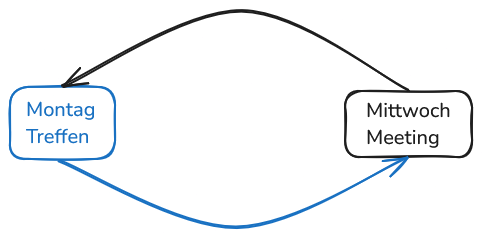
\includegraphics[width=0.6\linewidth]{pictures/level1}
        \label{fig:lvl1}
    \end{figure}
\end{frame}

\begin{frame}{Problem: Programmieren beim Montag Treffen}
    \begin{figure}
        \centering
        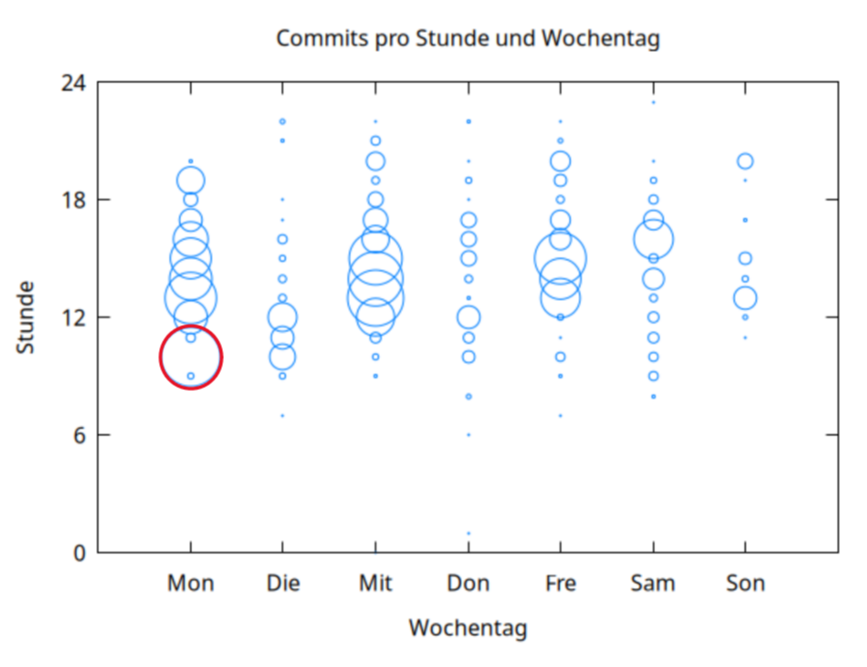
\includegraphics[width=0.52\linewidth]{pictures/hours}
        \label{fig:commit-hours}
    \end{figure}
\end{frame}

\subsection{1. Verbesserung}
\begin{frame}{1. Verbesserung}
    \begin{figure}
        \centering
        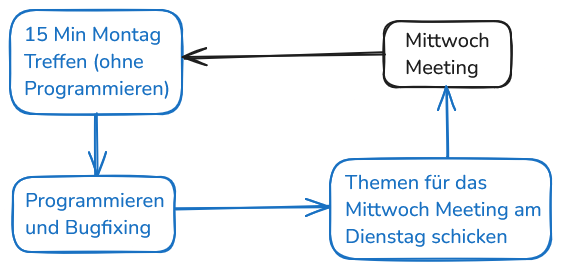
\includegraphics[width=0.6\linewidth]{pictures/level2}
        \label{fig:lvl2}
    \end{figure}
\end{frame}

\subsection{2. Verbesserung}
\begin{frame}{2. Verbesserung}
    \begin{figure}
        \centering
        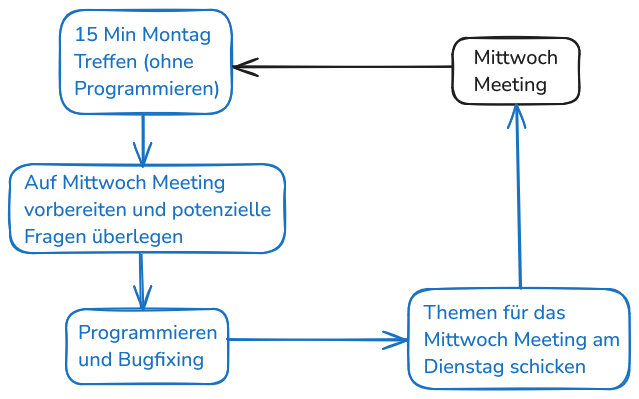
\includegraphics[width=0.6\linewidth]{pictures/level3}
        \label{fig:lvl3}
    \end{figure}
\end{frame}

\subsection{Wasserfallmodell}
\begin{frame}{Wasserfallmodell}
    \begin{itemize}
        \item Genutzt: Wasserfallmodell mit Rückkopplung
        \item Pros:
        \begin{itemize}
            \item Produktdefinition klar für alle
            \item Hohe Codequalität
        \end{itemize}
        \item Cons:
        \begin{itemize}
            \item Dokumentation aufwendig
            \item Rückkopplung nicht immer effizient
        \end{itemize}
    \end{itemize}
\end{frame}
%!TEX root = ../presentation.tex
\section{Werkzeuge}

\subsection{Workflow}
\begin{frame}{Größe}
    \begin{itemize}
        \item 103 Issues
        \item 124 Pull Requests
        \item 1243 Commits
        \item 9234 Zeilen Code
    \end{itemize}
\end{frame}

\begin{frame}[plain]
    \thispagestyle{plain}
    \begin{figure}
        \centering
        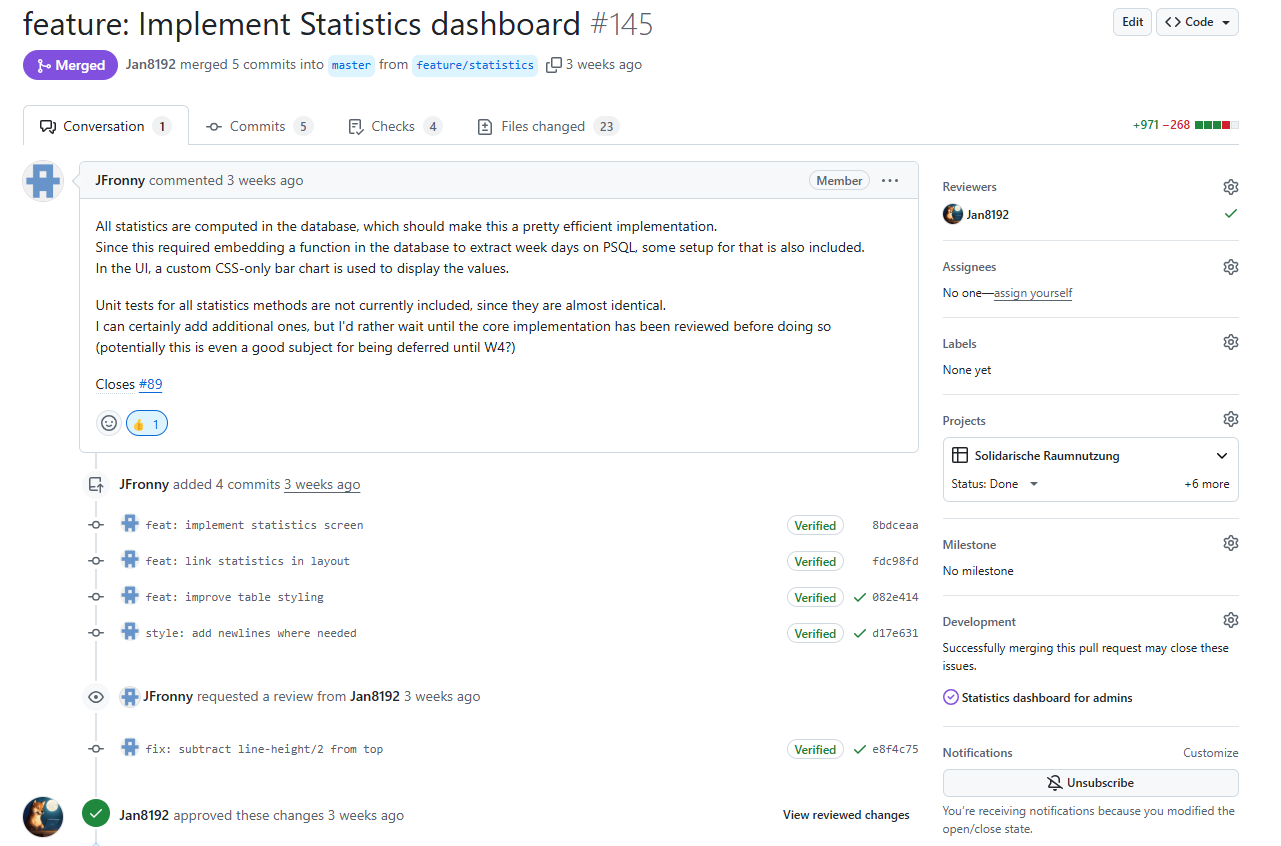
\includegraphics[width=1\linewidth]{pictures/pr_reviews}
        \label{fig:pr_reviews}
    \end{figure}
\end{frame}

\subsection{Qualität}
\begin{frame}{Unit Tests}
    \begin{columns}
        \column{.5\linewidth} \begin{itemize}
            \item 195 Unit und Integration Tests
            \item JUnit
            \item Mockito
            \item JaCoCo
        \end{itemize}
        \column{.5\linewidth} \begin{table}[h]
            \centering
            \renewcommand{\arraystretch}{1.3}
            \begin{tabular}{l|c}
                \textbf{Paket} & \textbf{Line Coverage} \\
                \hline
                \hline
                \textit{Controller}  & 77\% \\
                \textit{Domain}      & 91\%\\
                \textit{DTO}         & 83\%\\
                \textit{Filter}      & 90\% \\
                \textit{Repository}  & 100\% \\
                \textit{Service}     & 84\% \\
                \hline
                \textit{Gesamt}      & 76\% \\
            \end{tabular}
            \caption{Coverage der verschiedenen Pakete}
            \label{tab:progress}
        \end{table}
    \end{columns}
\end{frame}

\begin{frame}{CI}
    \begin{columns}
        \column{.5\linewidth} \begin{itemize}
            \item 195 Unit und Integration Tests
            \item JUnit
            \item Mockito
            \item JaCoCo
        \end{itemize}
        \column{.5\linewidth} \begin{figure}
            \centering
            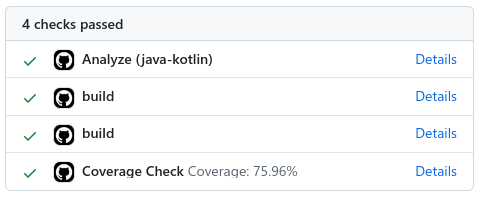
\includegraphics[width=1\linewidth]{pictures/pr_actions}
            \label{fig:pr_actions}
        \end{figure}
    \end{columns}
\end{frame}
%!TEX root = ../Pflichtenheft.tex
\section{Funktionen}

\subsection{Erster Unterabschnitt}
\begin{frame}{Blöcke}{in den KIT-Farben}
    This is a frame. content here.
\end{frame}

\subsection{Zweiter Unterabschnitt}
\begin{frame}{Auflistungen}
    More content here.
\end{frame}

%!TEX root = ../Pflichtenheft.tex
\section{Live-Demo}

\subsection{Erster Unterabschnitt}
\begin{frame}{Blöcke}{in den KIT-Farben}
    This is a frame. content here.
\end{frame}

\subsection{Zweiter Unterabschnitt}
\begin{frame}{Auflistungen}
    More content here.
\end{frame}

\section{Fragen?}


\end{document}
